\chapter{Test Automation AIs}

Testing software is an incredibly important factor when talking about software quality, it's objective is to verify that the code structure works as intended while also detecting problems before deployment. However, traditional testing procedures are usually time-consuming, require a lot of work, and are difficult to maintain especially in today's age where software systems keep rapidly evolving. Because of this, test automation has become a necessary component in modern programming.

Recently, AI has been introduced to test automation with the main objective of improving the effectiveness of such tests, while also reducing the effort required. AI test automation tool use various techniques, such as machine learning and pattern recognition to create, execute, and maintain test cases.

Software quality wise, test automation AIs have the possibility of increasing test coverage and enhancing the detection of problems. On the other hand, the use of these tools brings forward new hardships, such as an appropriate and in-depth validation of the test results by a human and the risk of relying on the tools too much. Knowing both the pros and cons of test automation AIs is necessary when we look at the impact it'll have on software quality.

\begin{table}[h]
\small
\centering
\caption{Feature-based comparison of selected Test Automation AIs}
\resizebox{1\textwidth}{41pt}{
\begin{tabular}{|c|c|c|c|}
\hline
\textbf{Feature} & \textbf{mabl} & \textbf{Testim} & \textbf{Testsigma}\\
\hline
\textbf{Primary purpose} & End-to-end web testing & End-to-end web \& mobile testing & End-to-end web \& mobile testing \\
\hline
\textbf{AI Usage} & Test generation & Smart locators & NLP-based test execution \\
\hline
\textbf{Test types supported} & Functional, regression & Functional, regression & Functional, regression \\
\hline
\textbf{Developer control} & Medium & High & Medium \\
\hline
\textbf{Accessibility} & Medium & Medium-high & High \\
\hline
\textbf{Suited for} & Automated regression pipelines & Controlled AI testing & Accessible test automation \\
\hline
\end{tabular}
}
\label{table_5.1}
\end{table}

\newpage

\section{Mabl}

Mabl is an AI-native test automation platform founded in 2016, with the objective of empowering software teams to deliver high quality software. \cite{mabl} Using its CLI developers can execute tests locally, this lets them get sooner during programming a feedback before their work is merged on the main branch of a project.


\begin{figure}[H]
    \centering
    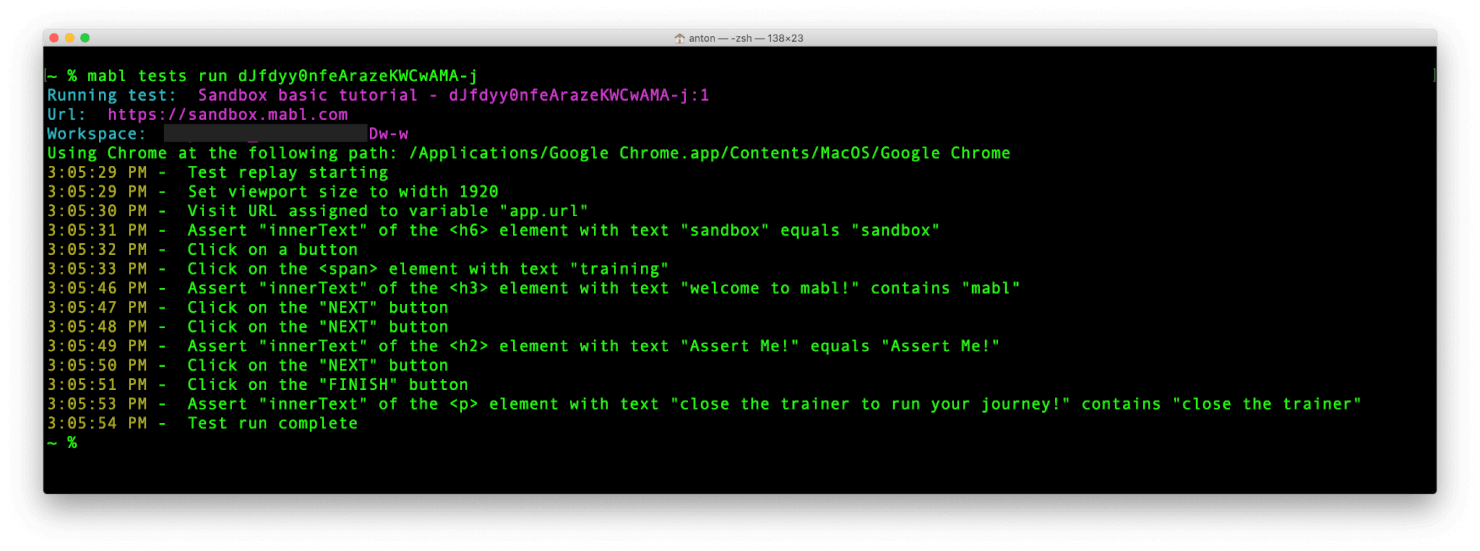
\includegraphics[width=0.95\linewidth]{images/mabl1.png}
    \caption{Executing and monitoring tests from terminal with mabl CLI \cite{what_is_mabl}}
    \label{fig:mabl_1}
\end{figure}

One of the main features of mabl is how it uses AI techniques to adapt test cases to changes in the program while testing. Through various mechanisms, mabl has the ability to modify codes in which UI elements might be changing reducing how fragile a test might be. In addition to that, mabl can create a customized test automatically based on the user's interactions or necessities.

When viewed under how it impacts on software quality, mail's main objective is to make sure that the reliability and regression testing effectiveness is improved. Since it maintains the test validity long-term it makes sure that if there is a change in the source code it wont lead to unwanted side effects. However, programmers could understand the test logic less because of the \textit{abstraction} that mabl offer, which means that a careful validation of the results is mandatory.

In the end, even though mabl offers some great advantages we should also look at the limitations it comes with. Relying too much on an automated test generator could make it so that programmers aren't in control of ho the tests behave, especially in more complex scenarios. In addition to that, an oversight of quality of the data used to train the AI is necessary to increase its effectiveness.

\section{Testim}

Testim is a full-featured test automation platform, launched in the late 2014 and with the objective of turning the mundane procedure of hand writing end-to-end tests into an AI-based functional test automation solution\cite{what_is_testim}. It's designed to be integrated in today's development cycles, supporting constant testing.

\begin{figure}[H]
    \centering
    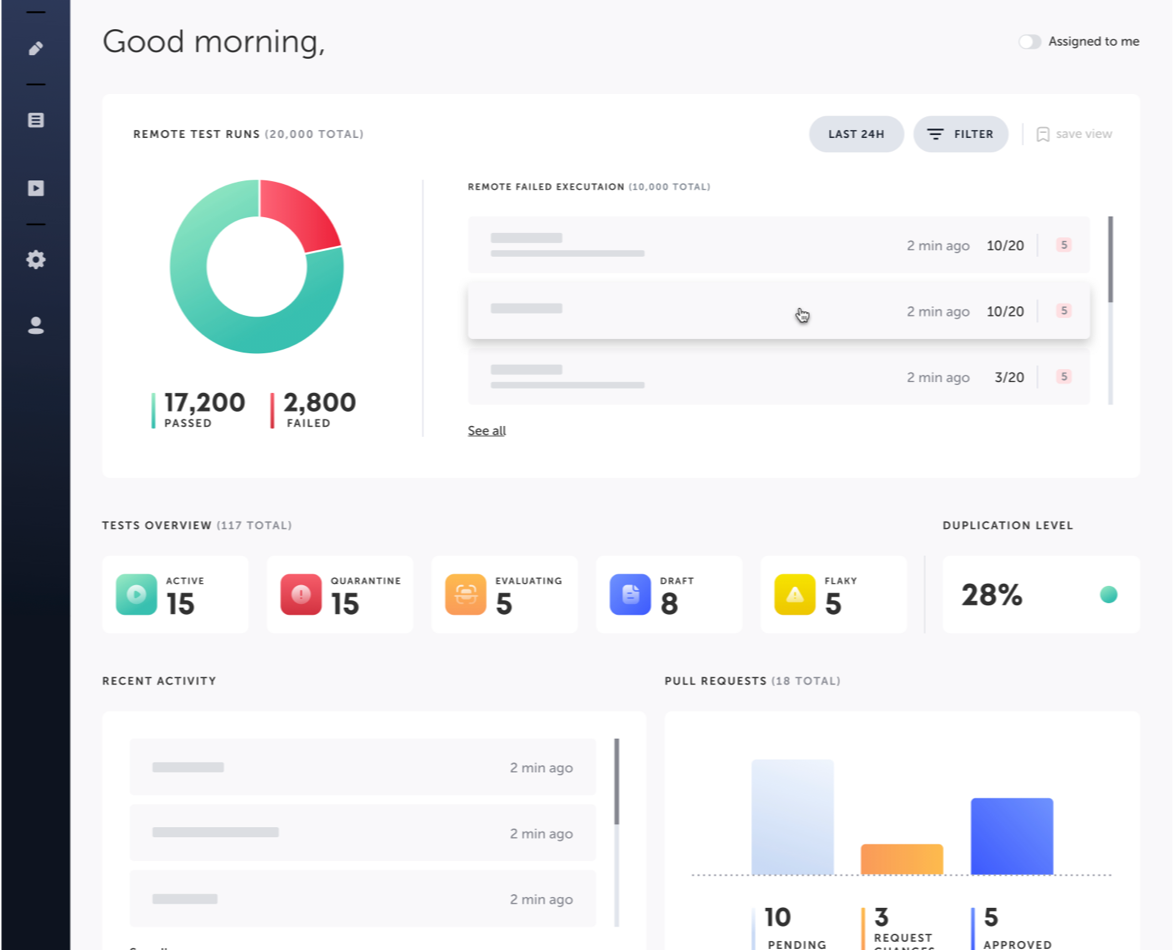
\includegraphics[width=0.55\linewidth]{images/dashboard_carousel@2x-1174x950.png}
    \caption{Testim UI \cite{testim_ui}}
    \label{fig:testim_1}
\end{figure}

It uses AI locators which make the creation of tests an easier task while also keeping them working when the source code gets modified. In addition to that, customized locators, that are made specifically for your application, are also one of the main methods used by Testim. It can also group automatically for reusable modules, for example it can save time with the creation and maintaining of duplicate tests and also identify steps that are repeated and can then be reused. \cite{what_testim_does}

Software quality wise, Testim contributes on making automated tests while making sure their reliability and maintainability is improved. It can reduce the amount of false-alarms when an interface change is done since it supports a stable regression testing process. Another positive is that Testim lets you customize the logic behind a test which lets programmers remain in control, unlike other test automation AIs.

Even though Testim has many advantages, there also are some important limitations to be taken in consideration. While the previously mentioned locators can improve complex scenarios it still \textit{needs} manual scripting and some tuning by a human. Additionally the effectiveness is strictly dependent on the quality of the recorded test, highlighting how important the test design and validation is.

\section{Testsigma}

Testsigma is a test automation platform, launched in 2019, with the purpose of making automated testing for mobile apps, web testing, and APIs an easier task. It's main user base is composed of startups and product teams, making sure they're able to make and manage tests in plain English \cite{testsigma}.

\begin{figure}[H]
    \centering
    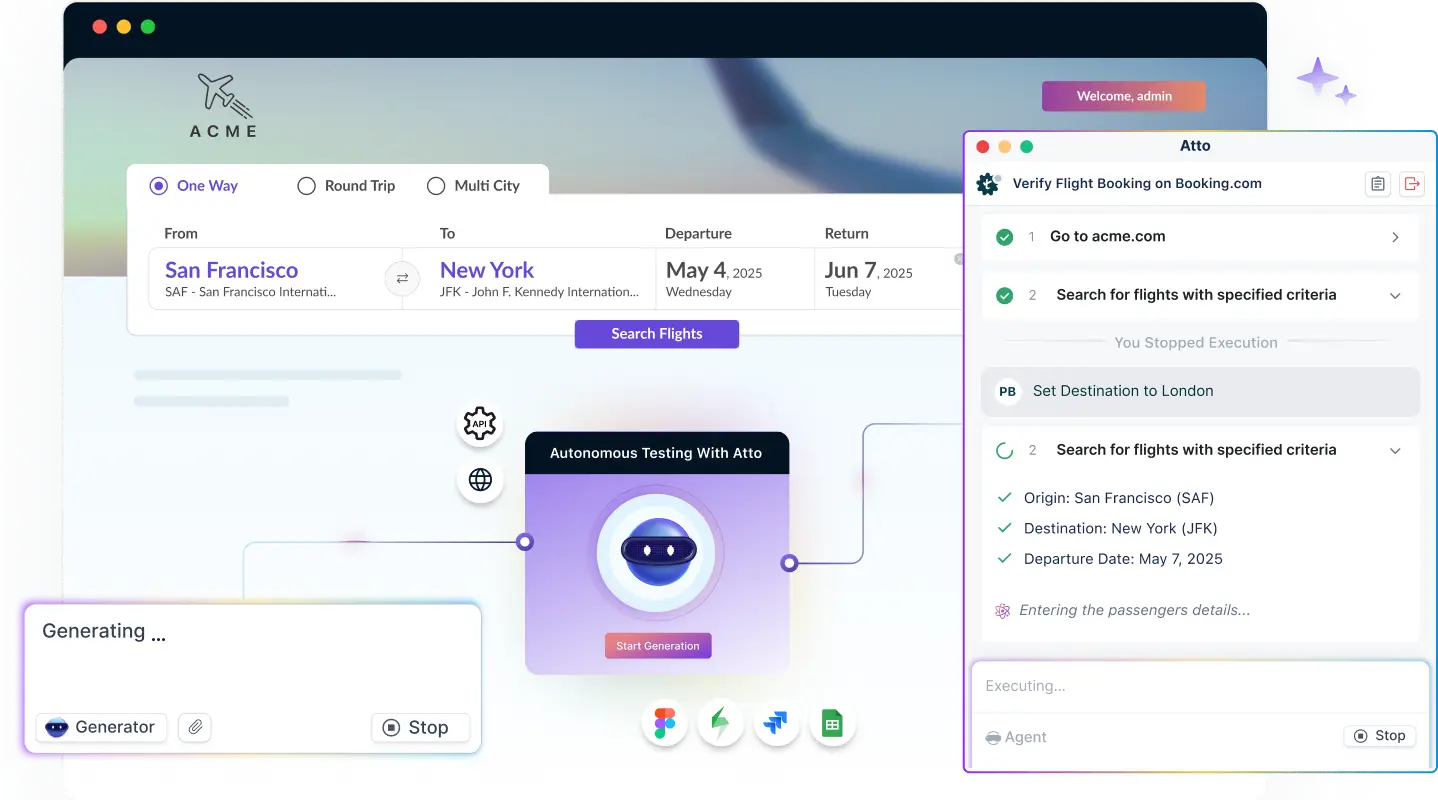
\includegraphics[width=0.77\linewidth]{images/ai-web-testing.png}
    \caption{Testsigma UI with an example of English written test \cite{testsigma_ui}}
    \label{fig:testsigma_1}
\end{figure}

It applies AI to make test creation, execution, and maintenance an automatic procedure. Like we saw in the Figure \ref{fig:testsigma_1} the steps are written in a classic language (such as English), which means that the use of traditional scripting languages is reduced. Like Testim, it uses AI-based mechanisms to adapt the tests when the applications are modified, and it also supports cross-browser and platform testing with little to none intervention. \cite{testsigma}

When we talk about software quality, Testsigma supports an improved test coverage and consistency. Since it makes the test creation a less complex task, it enables a broader participation during the testing phase, which may lead to a higher number of validated scenarios. This helps detect bugs early on and also have more reliable regression testing.

On the other hand, using Testsigma comes with some limitations. Due to the natural languages prompts the control over the behavior of the test is reduced, making it not ideal for more complex scenarios. In addition to that, the excessive use of natural languages can limit the flexibility when compared to a script-based testing approach.